% Architecture of the gate: F (full image), B (M zeroed), C (41 length-and-flag features), unanimity gate.
% Compile:  pdflatex architecture.tex   ->  architecture.pdf, included by ../main.tex.
% Times fonts to match IEEEtran (which uses Times under pdfLaTeX).
\documentclass[tikz,border=2pt]{standalone}
\usepackage[T1]{fontenc}
\usepackage{mathptmx}
\usetikzlibrary{positioning,fit,backgrounds,arrows.meta,patterns,calc,decorations.pathreplacing,shapes.misc}

% Colours: grey for kept header bytes, red for M, white for zeroed addresses and ports.
\definecolor{hdr}{RGB}{150,150,150}
\definecolor{pay}{RGB}{225,225,225}
\definecolor{mfield}{RGB}{200,40,40}
\definecolor{guar}{RGB}{214,232,250}
\definecolor{atk}{RGB}{200,40,40}

\begin{document}
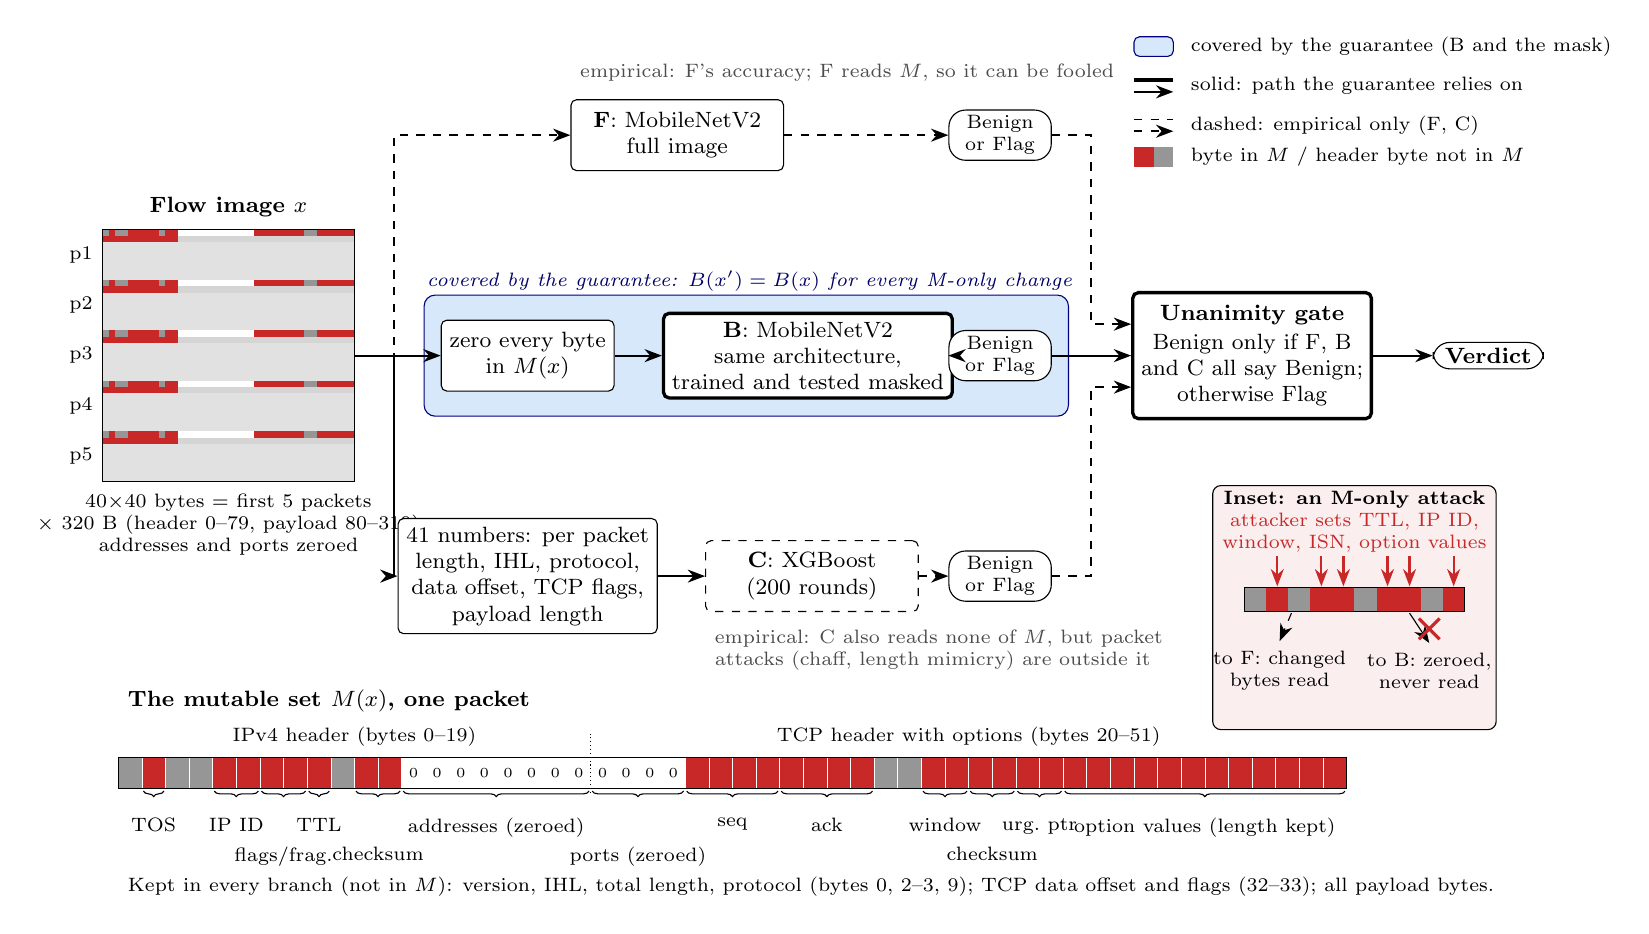
\begin{tikzpicture}[
  font=\footnotesize,
  >={Stealth[length=2.2mm]},
  box/.style={draw, rounded corners=2pt, align=center, minimum height=9mm, inner sep=3pt, fill=white},
  emp/.style={box, dashed},
  cert/.style={box, very thick},
  verd/.style={draw, rounded corners=6pt, align=center, inner sep=2pt, minimum width=13mm, fill=white, font=\scriptsize},
  flow/.style={->, thick},
  empflow/.style={->, thick, dashed},
]

% ------------------------------------------------------------ input image (40 x 40 bytes)
% 1 byte = 0.08 cm. Packet k occupies 8 rows; its first 2 rows (bytes 0-79) are the header.
\begin{scope}[shift={(0,3.6)}]
  \foreach \k in {0,...,4} {
    \fill[pay] (0, {3.2-0.64*(\k+1)}) rectangle (3.2, {3.2-0.64*\k-0.16});
    \fill[hdr] (0, {3.2-0.64*\k-0.16}) rectangle (3.2, {3.2-0.64*\k});
    % example IPv4 + TCP header with 12 option bytes: M bytes in red, address and port bytes white
    \foreach \b in {1,4,5,6,7,8,10,11,24,25,26,27,28,29,30,31,34,35,36,37,38,39,40,41,42,43,44,45,46,47,48,49,50,51} {
      \pgfmathtruncatemacro{\r}{\b/40}
      \pgfmathtruncatemacro{\c}{\b-40*\r}
      \fill[mfield] ({0.08*\c}, {3.2-0.64*\k-0.08*(\r+1)}) rectangle ({0.08*(\c+1)}, {3.2-0.64*\k-0.08*\r});
    }
    \foreach \b in {12,...,23} {
      \fill[white] ({0.08*\b}, {3.2-0.64*\k-0.08}) rectangle ({0.08*(\b+1)}, {3.2-0.64*\k});
    }
    \foreach \b in {52,...,79} {
      \pgfmathtruncatemacro{\r}{\b/40}
      \pgfmathtruncatemacro{\c}{\b-40*\r}
      \fill[hdr!40] ({0.08*\c}, {3.2-0.64*\k-0.08*(\r+1)}) rectangle ({0.08*(\c+1)}, {3.2-0.64*\k-0.08*\r});
    }
    \node[anchor=east, font=\scriptsize] at (0, {3.2-0.64*\k-0.32}) {p\the\numexpr\k+1\relax};
  }
  \draw (0,0) rectangle (3.2,3.2);
  \node[coordinate] (img-e) at (3.2,1.6) {};
  \node[coordinate] (img-hdr) at (0.4,3.12) {};
  \node[align=center, above=1pt, font=\footnotesize\bfseries] at (1.6,3.2) {Flow image $x$};
  \node[align=center, below=1pt, font=\scriptsize] at (1.6,0) {40$\times$40 bytes = first 5 packets\\$\times$ 320 B (header 0--79, payload 80--319)\\addresses and ports zeroed};
\end{scope}

% ------------------------------------------------------------ branches
\node[box, minimum width=27mm] (fbox) at (7.3,8.0) {\textbf{F}: MobileNetV2\\full image};

\node[box, minimum width=21mm] (mask) at (5.4,5.2) {zero every byte\\in $M(x)$};
\node[cert, minimum width=27mm, right=6mm of mask] (bbox) {\textbf{B}: MobileNetV2\\same architecture,\\trained and tested masked};

\node[box, minimum width=21mm] (feat) at (5.4,2.4) {41 numbers: per packet\\length, IHL, protocol,\\data offset, TCP flags,\\payload length};
\node[emp, minimum width=27mm, right=6mm of feat] (cbox) {\textbf{C}: XGBoost\\(200 rounds)};

% align F with B and C horizontally
\path (bbox.center |- fbox.center) coordinate (fpos);

\node[verd] (fo) at (11.4,8.0) {Benign\\or Flag};
\node[verd] (bo) at (11.4,5.2) {Benign\\or Flag};
\node[verd] (co) at (11.4,2.4) {Benign\\or Flag};

\node[box, very thick, minimum width=30mm, minimum height=16mm] (gate) at (14.6,5.2)
  {\textbf{Unanimity gate}\\[1pt] Benign only if F, B\\and C all say Benign;\\otherwise Flag};
\node[verd, minimum width=14mm, font=\footnotesize] (verdict) at (17.6,5.2) {\textbf{Verdict}};

% guarantee region: the mask and B
\begin{scope}[on background layer]
  \node[fill=guar, draw=blue!50!black, rounded corners=4pt, inner sep=6pt, fit=(mask)(bbox)(bo),
        label={[font=\scriptsize\itshape, text=blue!40!black, anchor=south west, inner sep=1pt]north west:covered by the guarantee: $B(x')=B(x)$ for every M-only change}] (gbox) {};
\end{scope}

% arrows
\draw[empflow] (img-e) -- ++(0.5,0) |- (fbox.west);
\draw[flow] (img-e) -- ++(0.5,0) |- (mask.west);
\draw[flow] (img-e) -- ++(0.5,0) |- (feat.west);
\draw[flow] (mask) -- (bbox);
\draw[flow] (feat) -- (cbox);
\draw[empflow] (fbox) -- (fo);
\draw[flow] (bbox) -- (bo);
\draw[empflow] (cbox) -- (co);
\draw[empflow] (fo.east) -- ++(0.5,0) |- ([yshift=4mm]gate.west);
\draw[flow] (bo.east) -- (gate.west);
\draw[empflow] (co.east) -- ++(0.5,0) |- ([yshift=-4mm]gate.west);
\draw[flow] (gate) -- (verdict);

\node[font=\scriptsize, text=black!70, align=left, anchor=north west] at ([yshift=-1mm]cbox.south west)
  {empirical: C also reads none of $M$, but packet\\attacks (chaff, length mimicry) are outside it};
\node[font=\scriptsize, text=black!70, align=left, anchor=south west] at ([yshift=1mm]fbox.north west)
  {empirical: F's accuracy; F reads $M$, so it can be fooled};

% ------------------------------------------------------------ zoom on one header: the mask M
% 52 bytes of an IPv4 + TCP header (IHL 20, data offset 32), 0.3 cm per byte.
\begin{scope}[shift={(0.2,-0.3)}]
  \def\w{0.3}
  \foreach \b in {0,...,51} { \fill[hdr] ({\w*\b},0) rectangle ({\w*(\b+1)},0.4); }
  \foreach \b in {1,4,5,6,7,8,10,11,24,25,26,27,28,29,30,31,34,35,36,37,38,39,40,41,42,43,44,45,46,47,48,49,50,51} {
    \fill[mfield] ({\w*\b},0) rectangle ({\w*(\b+1)},0.4);
  }
  \foreach \b in {12,...,23} { \fill[white] ({\w*\b},0) rectangle ({\w*(\b+1)},0.4); \node[font=\tiny] at ({\w*(\b+0.5)},0.2) {0}; }
  \foreach \b in {0,...,52} { \draw[white, line width=0.2pt] ({\w*\b},0) -- ({\w*\b},0.4); }
  \draw ({0},0) rectangle ({\w*52},0.4);
  \draw[densely dotted] ({\w*20},-0.05) -- ({\w*20},0.7);
  \node[font=\scriptsize, anchor=south] at ({\w*10},0.42) {IPv4 header (bytes 0--19)};
  \node[font=\scriptsize, anchor=south] at ({\w*36},0.42) {TCP header with options (bytes 20--51)};
  % field labels under the strip
  \foreach \a/\b/\t/\y in {1/1/TOS/-0.25, 4/5/IP ID/-0.25, 6/7/{flags/frag.}/-0.62, 8/8/TTL/-0.25, 10/11/checksum/-0.62,
                          12/19/addresses (zeroed)/-0.25, 20/23/ports (zeroed)/-0.62, 24/27/seq/-0.25, 28/31/ack/-0.25,
                          34/35/window/-0.25, 36/37/checksum/-0.62, 38/39/urg.\ ptr/-0.25, 40/51/option values (length kept)/-0.25} {
    \draw[decorate, decoration={brace, mirror, amplitude=2pt}] ({\w*\a+0.02},-0.03) -- ({\w*(\b+1)-0.02},-0.03);
    \node[font=\scriptsize, anchor=north] at ({\w*(\a+\b+1)/2},\y) {\t};
  }
  \node[font=\scriptsize, anchor=north west, align=left] at (0,-1.0)
    {Kept in every branch (not in $M$): version, IHL, total length, protocol (bytes 0, 2--3, 9); TCP data offset and flags (32--33); all payload bytes.};
  \node[font=\footnotesize\bfseries, anchor=south west] at (0,0.85) {The mutable set $M(x)$, one packet};
\end{scope}

% ------------------------------------------------------------ attacker inset
\begin{scope}[shift={(15.7,0.75)}]
  \node[draw, rounded corners=3pt, fill=atk!8, minimum width=36mm, minimum height=31mm] (inset) at (0.2,1.25) {};
  \node[font=\scriptsize\bfseries, anchor=north] at (0.2,2.85) {Inset: an M-only attack};
  \node[font=\scriptsize, align=center, text=atk] (att) at (0.2,2.2) {attacker sets TTL, IP ID,\\window, ISN, option values};
  % mini header row: grey kept, red M
  \foreach \b/\c in {0/hdr,1/mfield,2/hdr,3/mfield,4/mfield,5/hdr,6/mfield,7/mfield,8/hdr,9/mfield} {
    \fill[\c] ({-1.2+0.28*\b},1.2) rectangle ({-1.2+0.28*(\b+1)},1.5);
  }
  \draw (-1.2,1.2) rectangle (1.6,1.5);
  \foreach \b in {1,3,4,6,7,9} { \draw[->, atk, thick] ({-1.06+0.28*\b},1.9) -- ({-1.06+0.28*\b},1.52); }
  \node[font=\scriptsize, align=center] (tof) at (-0.75,0.45) {to F: changed\\bytes read};
  \node[font=\scriptsize, align=center] (tob) at (1.15,0.45) {to B: zeroed,\\never read};
  \draw[->, dashed] (-0.6,1.18) -- (tof.north);
  \draw[->] (0.9,1.18) -- (tob.north);
  \node[draw, very thick, atk, cross out, minimum size=2.2mm, inner sep=0pt] at (1.15,0.98) {};
\end{scope}

% ------------------------------------------------------------ legend
\begin{scope}[shift={(13.1,7.75)}]
  \fill[guar, draw=blue!50!black, rounded corners=2pt] (0,1.25) rectangle (0.5,1.5);
  \node[anchor=west, font=\scriptsize] at (0.6,1.375) {covered by the guarantee (B and the mask)};
  \draw[very thick] (0,0.95) -- (0.5,0.95); \draw[->, thick] (0,0.8) -- (0.5,0.8);
  \node[anchor=west, font=\scriptsize] at (0.6,0.875) {solid: path the guarantee relies on};
  \draw[dashed] (0,0.45) -- (0.5,0.45); \draw[->, thick, dashed] (0,0.3) -- (0.5,0.3);
  \node[anchor=west, font=\scriptsize] at (0.6,0.375) {dashed: empirical only (F, C)};
  \fill[mfield] (0,-0.15) rectangle (0.25,0.1); \fill[hdr] (0.25,-0.15) rectangle (0.5,0.1);
  \node[anchor=west, font=\scriptsize] at (0.6,-0.025) {byte in $M$ / header byte not in $M$};
\end{scope}

\end{tikzpicture}
\end{document}
